\chapter[Introdução]{Introdução}

	\section[Problema]{Problema}

	Tirar chope é uma arte.  Não há muito que se discutir, ao se conversar com 
	apreciadores \textit{sommeliers} do mesmo, eles hão de concordar que isso 
	deve ser feito com paixão, dedicação  e técnica,  para que se obtenha o máximo de 
	qualidade. Requisitos que muitas vezes não são cumpridos por aqueles que servem o
	chope como emprego.
	
	Dado o custo  envolvido com o trabalho de garçons, demora no atendimento,
	falta de praticidade, ausência de padronização na tiragem do chope e problemas de
	controle de temperatura, os quais contribuem para a desvalorização do produto,
	prejudicam o seu consumo, bem como encarecem o mesmo, deseja-se 
	minimizar as ocorrências do que  foi citado. 	
	
	\section[Estado da Arte]{Estado da Arte}
	
	No mundo inteiro, a cada dia, mais e mais pessoas se deixam seduzir pelo insuperável sabor das bebidas fermentadas, como a cerveja, e particularmente o chope. Assim sendo esse permite a existência de um mercado que estimule a criatividade de muitos empreendedores.  

	Hodiernamente a bebida é um atrativo para casas noturnas e eventos que ao longo dos anos ganhou vários apreciadores,possuindo inclusive eventos voltados apenas para os degustadores da bebida. 

	Um exemplo é o sistema myTapp de uma startup de Florianópolis.  O sistema faz a venda de chope ao estilo 
	\textit{self-service}, no qual os usuários compram créditos para uso da máquina e podem colocar somente a quantidade que 
	consumirem. Esse sistema favorece novatos no consumo de chope que têm a oportunidade de serem cobrados somente 
	pelo que consumirem, podendo provar diversos tipos de chope. A figura \ref{exemplo-chopp} mostra o uso desse sistema.

	\begin{figure}[H]
		\centering
		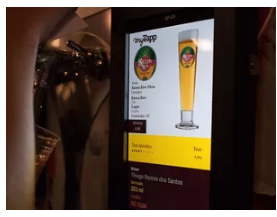
\includegraphics[scale= 0.9]{figuras/exemplo-chopp.png}
		\caption{Exemplo de chopeira automatizada.}
		\label{exemplo-chopp}
	\end{figure}

	Outro exemplo de equipamento de ponta é uma chopeira  que se encontra no Japão. Ela é capaz de servir de forma 
	automática os copos e localiza-se no Aeroporto Internacional de Kansai (KIX) em Osaka. A foto da mesma encontra-se 
	na imagem \ref{exemplo-japao}.

	\begin{figure}[!htb]
		\centering
		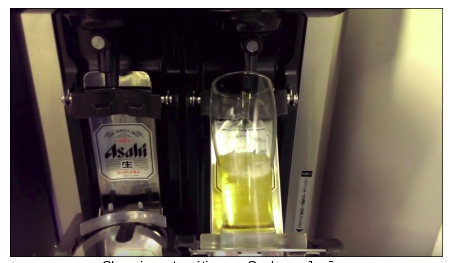
\includegraphics[scale= 0.9]{figuras/exemplo-japao.png}
		\caption{Exemplo de chopeira automatizada.}
		\label{exemplo-japao}
	\end{figure}

	\section[Objetivos]{Objetivos}
		\subsection[Geral]{Geral}
			Construir uma chopeira que realiza a venda e a tiragem de chopp de forma automatizada, seguindo o 
			paradigma de uma \textit{Vending Machine}. 

		\subsection[Específico]{Específico}
			\begin{itemize}
				\item Servir automaticamente o chope.
				\item Comprovar autenticação da compra previamente efetuada.
				\item Efetivar a compra  de forma online. 
				\item Realizar o controle e monitoramento eletrônico de temperatura de forma automatizada.
				\item Inclinar o copo, de acordo com os padrões de tiragem de chope.
				\item Controlar a quantidade de espuma no copo (colarinho) de acordo com a escolha do usuário e padrões predefinidos .
				\item Selecionar a quantidade de chope a ser servida, de acordo com padrões prévios.
				\item Fornecer energia de forma suplementar em casos emergenciais.
				\item Permitir a escolha entre dois tipos de chope
			\end{itemize}
	
	\section[Escopo]{Escopo}
		Trata-se de uma solução de venda remota para compra de chope no cartão, servindo com preferências predefinidas 
		(colarinho, quantidade e tipo), realizando a venda de forma autônoma otimizando a tiragem do chope.Essa 
		solução é obtida a partir de um sistema que possui alimentação redundante de energia por um certo período de 
		tempo, fazendo parte de um sistema para controle da quantidade e das vendas de chope. O escopo não engloba a o 
		congelamento do chope; a produção do chope ou de seu gás; a venda de drinks, cerveja, refrigerantes e 
		alimentos; o pagamento via dinheiro em espécie; uma máquina outdoor; a troca automática do chope (feito 
		manualmente) e o reuso do copo, assumindo que os copos que serão consumidos serão reusados.

	\section[Termo de Abertura do Projeto]{Termo de Abertura do Projeto}
		O Termo de Abertura de Projeto objetiva formalizar o início do projeto AutoChope, onde ocorrerá o planejamento 
		inicial de custos, restrições, riscos, tempo, cronograma e marcos. 

		\subsection[Descrição do Projeto]{Descrição do Projeto}
			Para ter uma visão clara do projeto, foi usado o mapeamento de atividade no modelo 5W2H, que está descrito 
			a seguir:
			\begin{enumerate}
				\item \textit{What?}
					\begin{itemize}
						\item Uma \textit{vending-machine} de chope;
						\item Uma máquina como serviço
					\end{itemize}
				\item \textit{Why}?
					\begin{itemize}
						\item Reduzir custos com mão de obra;
						\item Praticidade para servir o chop;
						\item Praticidade na compra e consumo;
						\item Facilidade em gerenciar o consumo;
						\item Agregar valor com Inovação e tecnologia	
					\end{itemize}
				\item \textit{Where}?
					\begin{itemize}
						\item No campus Gama da faculdade de Brasília;
						\item República Kzona;
						\item Galpão da FGA;
						\item Laboratório NEI;
						\item Laboratório de Materiais
					\end{itemize}
				\item \textit{When}?
					\begin{itemize}
						\item No período do segundo semestre de 2017
					\end{itemize}
				\item \textit{Who}?
					\begin{itemize}
						\item Alunos dos Cursos de Engenharias da Universidade de Brasília Campus Gama que cursam a 	disciplina Projeto Integrador 2
					\end{itemize}
			\end{enumerate}

			\begin{enumerate}
				\item \textit{How}?
					\begin{itemize}
						\item Cada engenharia define
					\end{itemize}
				\item \textit{How Much}?
					\begin{itemize}
						\item A pensar
					\end{itemize}
			\end{enumerate}

		\subsection[Propósito e justificativa do Projeto]{Propósito e justificativa do Projeto}
		
		\subsection[Restrições do Projeto]{Restrições do Projeto}
			Legislação
			\textit{De acordo com a legislação brasileira, especificamente o ECA (Estatuto da Criança e do Adolescente), é crime contra a criança e o adolescente, por ação ou omissão, sem prejuízo do disposto na legislação penal: “vender, fornecer, servir, ministrar ou entregar, ainda que gratuitamente, de qualquer forma, a criança ou a adolescente, bebida alcoólica ou, sem justa causa, outros produtos cujos componentes possam causar dependência física ou psíquica”. Tal crime tem pena de detenção de 2 (dois) a 4 (quatro) anos, e multa, se o fato não constitui crime mais grave. Além disso, a lei ainda se refere expressamente a proibição da venda de bebidas alcoólicas à criança ou ao adolescente, estabelecendo pena: de multa de R$ 3.000,00 (três mil reais) a R$ 10.000,00 (dez mil reais) e de medida administrativa de interdição do estabelecimento comercial até o recolhimento da multa aplicada. Dessa forma, toda a construção do projeto deve levar em conta que não será possível vender chope aos menores de idade.
			}

		\subsection[Riscos do Projeto]{Riscos do Projeto}

		\subsection[Custos do Projeto]{Custos do Projeto}

		\subsection[\textit{Stakeholders}]{\textit{Stakeholders}}

			\subsubsection[Cliente]{Cliente}
			
			\subsubsection[Equipe de Gerência]{Equipe de Gerência}

			\subsubsection[Equipe de Desenvolvimento]{Equipe de Desenvolvimento}

			\subsubsection[Docentes]{Docentes}

		\subsection[Produto do Projeto]{Produto do Projeto}


